\begin{figure}[!ht]
    \centering
    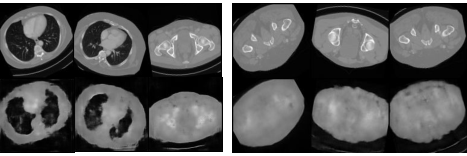
\includegraphics[width=\linewidth]{pics/2_equiv_vae/eqvae_vae_cs_recon_unk_rot.pdf}\hfill
    \caption{Example of reconstructed images using Eq-VAE (left-3) and VAE (right-3) as a prior. The top row shows ground truth rotated images prior to measurement, and the bottom row shows the corresponding CS reconstructed images. We notice in the third column (both left and right images), the VAE reconstructed image is $180^{\circ}$ rotated with respect to the canonical configuration while the Eq. VAE is able to retrieve the configuration effectively.}
    \label{fig:mayo_eqvae_vae_rec_unk}
\end{figure}
